\documentclass[letterpaper, 12 pt]{amsart}
\usepackage[margin=1in]{geometry}
\usepackage{amsmath} % assumes amsmath package installed
\usepackage{amssymb}  % assumes amsmath package installed
\usepackage{todonotes}

% NEW COMMANDS
\newcommand{\hoj}[1]{\todo[inline,color=blue!20]{#1}}
\newcommand{\ram}[1]{\todo[inline,color=red!20]{#1}}
\newcommand{\R}{\mathbb{R}}

% NEW THEOREM ENVIRONMENTS
\newtheorem{thm}{Theorem}[section]
\newtheorem{defn}[thm]{Definition}
\newtheorem{prop}[thm]{Proposition}
\newtheorem{cor}[thm]{Corollary}
\newtheorem{lem}[thm]{Lemma}
\newtheorem{ass}[thm]{Assumption}


% MATH OPERATORS
\DeclareMathOperator{\Diff}{Diff}
\DeclareMathOperator{\Fr}{Fr}
\DeclareMathOperator{\GL}{GL}
\DeclareMathOperator{\Dens}{Dens}
\DeclareMathOperator{\pr}{pr}

\title{
  A 
  multiscale
  advection scheme for
  densities on manifolds
}

\author{Henry O. Jacobs and Ram Vasudevan}% <-this % stops a space

\begin{document}

\maketitle

\begin{abstract}
  The task of computing a probability density advected by an 
  dynamical system may be viewed as an inifinite dimensional problem
  on the positive cone of the unsigned densities.
  Existing schemes exhibit numerical artifacts such as
  ``negative probabilities'' and have restricted convergence results.
  In this article we present a convergent method
  which preserves the positivity of probability densities
  at arbitrarily low resolutions.
  Moreover, we can use a single dense chart to transport the machinary of wavelet analysis to a manifolds.
  This allows us to avoid the use of transition maps between multiple charts, and to implement our method on a variety of non-Euclidean spaces at multiple length scales with existing wavelet algorithms designed on $\R^n$.
\end{abstract}


%%%%%%%%%%%%%%%%%%%%%%%%%%%%%%%%%%%%%%%%%%%%%%%%%%%%%%%%%%%%%%%%%%%%%%%%%%%%%%%%
\section{Introduction}
  The task of advecting a probability density presents itself
  in a variety of scenarios.
  Engineers are often presented
  with dynamical systems and incomplete knowledge
  of the initial conditions.
  If there is some region, $S$, of state-space which is ``dangerous''
  he or she may wish to compute the probability of landing
  in this dangerous region at time $T$.
  If the initial condition is given in the form of a
  probabilty density $p(\cdot \mid t=0)$
  the probability of landing in $S$ at time $T$
  is $P( x \in S \mid t = T)  = \int_S p( dx | t=T )$
  where $p(dx|t=T)$ is the advected probability density at time $T$.
  In order to compute $p(dx\mid t=T)$
  one must advect $p(dx\mid t=0)$ under the flow of the dynamics.

\subsection{Background material}
  Let $p_0$ be a probability density on $\R^n$
  and let $X$ be a vector-field on $\R^n$.
  We denote the flow of $X$
  by $\Phi_X^t$.
  We can define the time-dependent probability
  density $p$ by
  \begin{align}
    p( x ; t) = 
    \left| \det\left[ D\Phi_X^t(x) \right] \right|^{-1} p_0\left( \left[\Phi_X^t\right]^{-1}(x) \right), \label{eq:push_forward}
  \end{align}
  where $D\Phi_X^t(x)$ is the Jacobian matrix of
  $\Phi_X^t$ at the point $x \in \R^n$.
  The density $p(x;t)$ represents how the density
  $p_0(x)$ transforms under the flow of $X$.
  We observe that $p(x;0) = p_0(x)$ and, upon taking
  a time derivative,
  \begin{align}
    \partial_t p (x;t) + \partial_i (X^i p)(x) = 0 \label{eq:Louiville}
  \end{align}
  for all $x \in \R^n$.
  Equation \eqref{eq:Louiville} is known as the \emph{Louiville equation}.
  Using \eqref{eq:push_forward} to compute $p$ is difficult
  because $\Phi_X^t$ is typically a non-linear map with no closed
  form expression.
  To compute $p( x ; t)$, it is often easier
  to numerically solve \eqref{eq:Louiville}
  (a first order linear evolution PDE)
  with the initial condition $p_0$.
  On a manifold $M$, the advection equation is a linear
  evolution PDE involving the Lie-derivative
  where the description in a local coordinate chart is
  given by \eqref{eq:Louiville}.
  This will be addressed in \S \ref{sec:math} (see \eqref{eq:advection}).

\subsection{A naive psuedo-spectral method}
\label{sec:naive}
  In this section we will present the simplest type of
  spectral discretization of \eqref{eq:Louiville}.
  Let $f^0,f^1,f^2,\dots \in L^2(\R^n)$ serve as an
  orthonormal Hilbert basis (e.g. a Fourier basis).
  Let $\rho(x,t)$ be the solution to \eqref{eq:Louiville}.
  Assuming $\rho(\cdot,t) \in L^2$ and $\partial_i X^i \in L^{\infty}$,
  we can define the scalars $\rho_j(t), A^k_j \in \R$
  by $\rho_j(t) = \langle \rho(\cdot ,t) , f^j \rangle_{L^2(\R^n)}$
  and $A^k_j = \langle (\partial_i X^i) f^j , f^k \rangle_{L^2(\R^n)}$.
  Then $\rho_j(t)$ satisfies the infinite-dimensional linear
  ordinary differential equation
  $
    \dot{\rho}_j = - \sum_{k=0}^{\infty}A^k_j \rho_k
  $.
  Moreover, $\rho(x,t) = \rho_j(t) f_j(x)$.
  We can truncate this system at some finite $N \in \mathbb{N}$
  to obtain an $N$-dimensional linear ordinary differential equation
  $\dot{\rho}_{N,j} = -\sum_{k=0}^{N} A^k_j \rho_{N,j}$ for $j=0,\dots,N$.
  It is notable that if $f_0,f_1,\dots$ is a Haar basis, then
  at finite resolution, this algorithm is equivalent to 
  partitioning the space into cells and the basis is equivalent
  to a set of indicator functions on the cells.
  The matrix $A^k_j$ is then simply a matrix of fluxes 
  known as a transfer operator.
  Under the right circumstances,
  this method converges as the cell width approaches $0$ and $N \to \infty$
  \cite{FroylandJungeKoltai2013}.

  However, for finite $N$, there is no guarantee that the reconstructed
  density $\tilde{\rho}(x,t) = \sum_{j=0}^N \rho_{N,j}(t) f_j(x)$
  is non-negative.
  Generically $\tilde{\rho}(x,t)$ will take on both signs, in
  contrast with the exact solution $\rho(x,t)$ (see figure \ref{fig:one_dim_system})
  Moreover, important entities such as the advected moments
  $\tilde{m}_i(t) = \int \tilde{\rho}(x,t) (\Phi_X^t)_*(f_i)dx$
  may fluctuate, also in contrast with the exact moments
  $m_i = \int \rho(x,t)  (\Phi_X^t)_*(f_i) dx$.
  When dealing with manifolds of even moderate dimensions
  (e.g. $d=3$) it is important for a method to behave well at finite $N$'s
  because it is infeasible to finely resolve along each dimension.

\subsection{Main contributions}
  In this paper we will present a method for advection of
  probability densities on manifolds.
  This method will yield reconstructed probability measures
  which are non-negative and mass conserving at any finite resolution.

\subsection{Notation}
  Manifolds, tangent bundles, vector fields, closure of a set (bar notation)

\section{Mathematical preliminaries}
\label{sec:math}
  Throughout this section we will have the following
  setup.  Let $M$ be a smooth manifold.
  We denote the tangent bundle of $M$ by $TM$.
  Given any $C^1$ function $f:M \to N$,
  we denote the tangent lift of $f$ by $Tf:TM \to TN$.

\subsection{Densities}
  A smooth density on $M$ is a smooth means of
  assigning real numbers to measureable sets.
  Hueristically, it is a map which
  takes an infinitesimal box (or volume element)
  on a manifold as input, and outputs the infinitesimal ``size''
  of the box (a real number).
  Therefore, in order to discuss densities,
  we must first mathematize the notion of an ``infinitesimal box.''
  This motivates our introduction of \emph{frames}.
  \begin{defn}
  \label{eq:frame_bundle}
    Given a manifold $M$, and a point $x \in M$,
    a \emph{frame at $x$} is a basis on the tangent space $T_x M$.
    We denote the set of frames at $x$ by $\Fr_x M$.
    The frame bundle is $\Fr M = \cup_{x \in M} \Fr_x M$.
  \end{defn}

  \begin{prop}
    There is a natural transitive
    action of $\GL(n)$ on each fiber of $\Fr M$.
  \end{prop}

  \begin{proof}
    Let $e = \{ e^1,\dots,e^n \} \in \Fr_x M$ for some $x \in M$.
    For each $A \in \GL(n)$ define the left action
    \begin{align*}
      A \cdot (e^1,\dots,e^n) := (A^j_1 e^j , \dots, A_n^j e^j ). 
    \end{align*}
    By inspection this actions is free and transitive.
    \footnote{This makes $\Fr M$ a $\GL(n)$ principal bundle over $M$.}
  \end{proof}

  Now that we understand frames (i.e. infinitesimal boxes)
  sufficiently well, we may introduce the notion of \emph{densities}.

  \begin{defn}[Appendix A \cite{BatesWeinstein1997}]
    \label{eq:density}
    Let $\alpha > 0$.
    An $\alpha$-\emph{density} on a manifold, $M$, is a map
    $\rho:\Fr M \to \R$ such that
    for any frame $e \in \Fr M$ and $A \in \GL(n)$,
    $
      \rho( A \cdot e ) =  | \det(A) |^\alpha \rho(e).
    $
    We denote the space of densities by $\Dens^\alpha(M)$.
    A $1$-density is simply called a \emph{density}, and
    so we denote $\Dens^1(M)$ by $\Dens(M)$.
    The integral of a density is defined via the same construction as that
    for $n$-forms \cite[Ch. 14]{Lee2006}.
    A \emph{mass density} is a density which is non-negative.
    and it is called a \emph{probability density} if its integral is
    unity.
  \end{defn}

  One can observe immediately that $\Dens^\alpha(M)$ is a vector-space.
  Despite this commonality with tensors,
  $1$-densities are \emph{not} tensors.
  Densities are very close in spirit to $n$-forms,
  but unlike $n$-forms, densities are \emph{non-oriented}
  due to the use of ``$|\det(A)|$'' rather than ``$\det(A)$'' 
  in the definition.
  Therefore, a density will not flip signs under a change of basis.
  This allows for the integral of a density to be well defined
  on non-orientable manifolds as well \cite[Ch. 14]{Lee2006}.

  \begin{prop}[Appendix A \cite{BatesWeinstein1997}]
    Let $\psi_1,\psi_2 \in \Dens^{1/2}(M)$.
    The function, $\psi_1 \psi_2$, obtained by
    scalar multiplication is a $1$-density.
    The pairing
    $
    \langle \psi_1, \psi_2 \rangle := \int_M \psi_1 \psi_2 
    $
    is a real inner-product.
    Finally, for any density $\rho$, the functions $\pm\sqrt{\rho}$ are
    $\frac{1}{2}$-densities.
  \end{prop}
  \begin{proof}
    Let $e \in \Fr M$ and $A \in \GL(n)$.
    We observe $\psi_1(A \cdot e) \psi_2(A \cdot e) = |\det(A) | \psi_1(e) \psi_2(e)$.  Thus $\psi_1 \psi_2 \in \Dens(M)$.
    Conversely $\pm \sqrt{\rho( A \cdot e)} = \pm | \det(A) |^{1/2} \sqrt{ \rho(e)}$. So $\pm \sqrt{\rho} \in \Dens^{1/2}(M)$.
    Finally, if $\psi \neq 0$ we see that $\| \psi \|^2 := \langle \psi , \psi \rangle \neq 0$.
    Thus $\langle \cdot , \cdot \rangle$ is weakly non-degenerate
    and defines an inner-product on $\Dens^{1/2}(M)$.
  \end{proof}

  Note that for any $C^1$ diffeomorphism $\Phi:M \to M$,
  there is a map $\Fr(\Phi) : \Fr M \to \Fr M$
  given by 
  ``$(e^1,\dots,e^n) \mapsto (T\varphi \cdot e^1, \dots, T\varphi \cdot e^n)$''.
  This defines the \emph{pull-back} of an $\alpha$-density
  $\nu \in \Dens^\alpha(N)$
  by $\Phi^* \nu := \nu \circ \Fr(\Phi) \in \Dens^\alpha(M)$.
  \begin{prop} \label{prop:isom}
    Let $\Phi \in \Diff(M)$.
    The transformation ``$\psi \mapsto \Phi^* \psi$'' for
    $\psi \in \Dens^{1/2}(M)$ is an isometry.
  \end{prop}
  \begin{proof}
    Let $\psi_1,\psi_2 \in \Dens^{1/2}(M)$ and observe
    \begin{align*}
      \langle \Phi^* \psi_1, \Phi^* \psi_2 \rangle
      = \int \Phi^*( \psi_1 \psi_2)
      = \int \psi_1 \psi_2
      = \langle \psi_1, \psi_2 \rangle,
    \end{align*}
    where the equivalence of the integrals follows
    from \cite[Proposition 14.32(c)]{Lee2006}.
  \end{proof}
  
  Given a vector field $X \in \mathfrak{X}(M)$
  we can denote the flow by $\Phi^t_X \in \Diff(M)$
  and define the Lie-derivative of an alpha density by
  $
    \pounds_X[ \nu ] := \left. \frac{d}{dt} \right|_{t=0} (\Phi_X^t)^* \nu.
  $
  This yields the following corollary to proposition \ref{prop:isom}.
  \begin{cor}
    For any $X \in \mathfrak{X}(M)$, $\pounds_X[ {}\cdot{} ]$
    is an anti-symmetric linear operator on $\Dens^{1/2}(M)$.
  \end{cor}
  With the Lie-derivative defined we can write the advection
  PDE for densities as
  \begin{align}
    \partial_t \nu + \pounds_X[\nu] = 0 \label{eq:advection},
  \end{align}
  for a time-dependent $\alpha$-density $\nu(t) \in \Dens^\alpha(M)$
  which is advected infinitesimally by the vector field 
  $X \in \mathfrak{X}(M)$.
  If $\alpha = 1$, \eqref{eq:advection} is written in local coordinates
  as \eqref{eq:Louiville}.

  Moreover, for a time-dependent half-density $\psi(t) \in \Dens^{1/2}(M)$
  equation \eqref{eq:advection} is written in local coordinates as
  \begin{align*}
    \partial_t \psi(x) 
    + X^i(x) \partial_i \psi(x) 
    + \frac{1}{2} (\partial_i X^i)(x) \psi(x) = 0.
  \end{align*}
  \begin{thm} \label{thm:advection}
    Let $\rho(t) \in \Dens(M)$ be a time-dependent probability density
    and let $\psi \in \Dens^{1/2}(M)$ be such that $\rho = \psi^2$.
    Assume that $\rho$ is $C^1$.
    Let $X \in \mathfrak{X}(M)$.
    The following are equivalent:
    \begin{enumerate}
      \item $\rho$ satisfies the advection equation \eqref{eq:advection} with $\alpha = 1$.
      \item $\psi$ satisfies the advection equation \eqref{eq:advection} with $\alpha = 1/2$.
    \end{enumerate}
  \end{thm}
  \begin{proof}
    Let $\psi$ satisfy \eqref{eq:advection}.
    We find
    \begin{align*}
      \partial_t (\psi^2) &= 2 \partial_t\psi \cdot \psi
      =-2 \pounds_X[\psi] \psi \\
      &= - 2 \left[ \left.\frac{d}{dt}\right|_{t=0}
         (\Phi_X^t)^* \psi \right] \cdot \psi \\
      &= - \left. \frac{d}{dt} \right|_{t=0}
        \left[ (\Phi_X^t)^* \psi \cdot (\Phi_X^t)^* \psi \right]\\
      &= - \left. \frac{d}{dt} \right|_{t=0}
        \left[ (\Phi_X^t)^* (\psi^2) \right] 
      = - \pounds_X[\psi^2].
    \end{align*}
    Therefore $\rho = \psi^2$ satisfies \eqref{eq:advection}.
    Conversely, if $\rho$ satisfies \eqref{eq:advection}
    and $\psi^2 = \rho$ then
    \begin{align*}
      \partial_t (\psi^2) = - \pounds_X[\psi^2] = - \pounds_X[\psi] \psi.
    \end{align*}
    Moreover, the right hand side is $2 (\partial_t \psi) \psi$.
    We can divide both side by $\psi$ at any point where $\psi(x) \neq 0$.
    By continuity of $\partial_t \rho$ and $\partial_t \psi$ we can
    verify \eqref{eq:advection} on the entire support of $\psi$
    (which is also the support of $\rho$).
    Outside the support it is neccesarily the case that
    $\rho = 0$ and  $\partial_i \rho = 0$.
    We observe that $\pounds_X[\rho] = 0$ as well.
    In this case $\pounds_X[\psi] = 0$ by the same argument.
    So we've verified \eqref{eq:advection} on the entire domain.
  \end{proof}

  We will use theorem \ref{thm:advection} later to justify building
  a numerical scheme to solve \eqref{eq:advection} with $\alpha = 1/2$
  in lieu of solving \eqref{eq:advection} with $\alpha = 1$.

\subsection{Euclidean realizations}
\label{sec:euclidean}
  We would like to apply wavelet theory later for the
  analysis and sparsity structure they provide.
  However, the notion of wavelets on manifolds is still young,
  and virtually all of the available wavelet analysis machinery
  is developed on Euclidean spaces and Tori.
  In this section we will present theorems which allow
  us to transform analysis on manifolds into problems
  of analysis on subspaces of functions on $\R^n$.

\begin{thm}
  \label{thm:Euclidean}
  Let $\varphi:U \subset M \to V \subset \R^n$ be a chart.
  As $\varphi$ is injective, we can invert it on the range $V$.
  If $U$ is dense in $M$ then the maps
  \begin{align*}
    f \in C^k(M) &\mapsto \varphi_*f = f \circ \varphi^{-1} \in C^k(V) \\
    \nu \in \Dens^\alpha(M) &\mapsto \varphi_* \nu = \nu \circ \Fr(\varphi^{-1}) \in \Dens^\alpha(V) \\
    X \in \mathfrak{X}(M) &\mapsto \varphi_* X = T\varphi \cdot X \circ \varphi^{-1} \in \mathfrak{X}(V)
  \end{align*}
  are injective ring/vector-space/Lie-algebra morphisms respectively.
  \end{thm}
  \begin{proof}
    Let $f,g \in C^k(M)$ be such that $\varphi_* f = \varphi_*g$.
    Assume $f \neq g$.
    Since the range of $\varphi^{-1}$ is $U$, it must be the case that
    $f(x) \neq g(x)$ for some $x \notin U$.
    As $U$ is dense in $M$ there is a sequence $x_0,x_1,\dots$ in $U$
    which converges to $x$.
    As $f$ and $g$ are continous $g(x_i) = f(x_i)$ must converge to a
    unique limit.  Thus $g(x) = f(x)$, contradicting the assumption
    that $f \neq g$.
    Therefore the map $f \in C^k(M) \to \varphi_* f \in C^k(V)$
    is injective.
    That it is a ring morphism can then be viewed directly, $\varphi_*(f) \cdot \varphi_*(g) = \varphi_*(f \cdot g)$ for any $f,g \in C^k(M)$.
    
    The same argument applies to vector-fields
    upon noting $\varphi_*(X+cY) = \varphi_*X + c \varphi_*Y$ for any $X,Y \in \mathfrak{X}(M)$ and $c \in \R$, and $\varphi_*([X,Y]) = [\varphi_*X, \varphi_*Y]$.

    Finally, the same argument applies to $\alpha$-densities
    upon noting $\varphi_*( \nu + c \mu) = \varphi_*\nu + c \varphi_* \mu$ for any $\nu,\mu \in \Dens^\alpha(M)$.
  \end{proof}
  
  \begin{cor}
    Assume the setup of theorem \ref{thm:Euclidean}.
    The map 
    ``$\psi \in \Dens^{1/2}(M) \mapsto \varphi_* \psi \in \Dens^{1/2}(V)$''
    is an isometry.
  \end{cor}
  \begin{proof}
    Simply observe
    \begin{align*}
      \langle \varphi_*\psi_1 , \varphi_*\psi_2 \rangle
      &= \int_V \varphi_*(\psi_1) \varphi_*(\psi_2) \\
      &= \int_V \varphi_*( \psi_1 \cdot \psi_2) \\
      &= \int_U \psi_1 \cdot \psi_2.
    \end{align*}
    As $U$ is dense in $M$, the above integral is unchanged by integration
    over $M$.   Thus we've verified $\langle \varphi_* \psi_1,\varphi_*\psi_2 \rangle = \langle \psi_1,\psi_2 \rangle$.
  \end{proof}

  The upshot of theorem \ref{thm:Euclidean} is that we may represent PDEs on manifolds
  as PDE's on Euclidean domains.
  In particular, theorem \ref{thm:Euclidean} equates the function
  space $C^k(M)$ with the subring
  \begin{align*}
    \varphi_*C^k(M) := \{ g \in C^k(V) \mid g = f \circ \varphi^{-1} , f \in C^k(M) \}.
  \end{align*}
  Thus any, PDE on $M$ can be fully represented as a PDE on a 
  subring of functions on $V$.
  

% \begin{thm} \label{thm:Euclidean}
%   Let $\varphi : V \subset \R^n \to U \subset M$ be a chart on 
%   a compact $C^k$-manifold $M$ such that $U$ is dense in $M$.
%   We can extend $\varphi$ to a surjective map
%   $\bar{\varphi}: \bar{V} \to M$ such that
%   $M$ is $C^k$-diffeomorphic to $\bar{V} / \bar{\varphi}$.
% \end{thm}
% \begin{proof}
%   Let $\{x_k\}$ we a sequence in $V$ which converges to the boundary
%   of $\bar{V}$, then $\varphi(x_k)$ converges to a unique point in
%   $M \backslash U$ because $M$ is compact and $\varphi$ is continous.
%   This extends $\varphi$ to the boundary of $\bar{V}$.

%   Observe that $\bar{\varphi}( \bar{V} ) = \bar{U} = M$.
%   By construction $\bar{\varphi}$ is injective on $\bar{V} / \bar{\varphi}$.
%   Thus $\bar{\varphi}$ is a bijection from $\bar{V} / \bar{\varphi}$ to $M$.
  
%   We have shown equivalence as sets.
%   To obtain equivalence as topological spaces use
%   the quotient topology induced by $\bar{\varphi}$.
%   To obtain $C^k$-equivalence, use the quotient topology
%   induced by the $k$th order jet of $\varphi$
%   and continuously extend to $\bar{V}$.
%   \footnote{This entails interpreting the $k$th order Taylor expansions
%   of $\varphi$ as  a map to the space of multidimensional polynomials.
%   We then apply the same argument used to prove equivalence as topological
%   spaces to this map.}
% \end{proof}

  As an example consider the $2$-sphere, $S^2 \subset \R^3$.
  If we use spherical coordinates we obtain a map
  $\varphi: (-\pi,\pi) \times (0,\pi) \to U \subset S^2$
  given by
  \begin{align*}
    \chi(\phi,\theta) = \begin{pmatrix}
      \cos(\phi) \sin(\theta) \\
      \sin(\phi) \sin(\theta) \\
      \cos(\theta)
      \end{pmatrix}.
  \end{align*}
  Then we find
  \begin{align*}
    &\varphi_*C^0(S^2) = \{
      f \in C^0( (-\pi,\pi)\times (0,\pi) \mid \\
    &\quad \begin{array}{l}
      \lim_{\theta \to 0} f(\phi,\theta) = f_{\rm north} \text{ for some } f_{\rm north} \in \R \\
      \lim_{\theta \to \pi} f(\phi,\theta) = f_{\rm south} \text{ for some } f_{\rm south} \in \R 
    \end{array}
    \}
  \end{align*}
  The canonical volume form on $S^2$ viewed as a subset of $\R^3$ is 
  given by
  \begin{align*}
    \mu_{S^2} = x dy \wedge dz - y dx \wedge dz + z dx \wedge dy.
  \end{align*}
  In spherical coordinates, this volume form is given by
  \begin{align*}
    \varphi_*(\mu_{S^2}) = \sin(\theta) d\theta \wedge d\phi.
  \end{align*}
  It is easy to observe that $|\mu_{S^2}|^\alpha \in \Dens^\alpha(M)$
  and arbitrary $\nu \in \Dens^\alpha(M)$ can always be written
  as $\nu = f_{\nu} \otimes |\mu_{S^2}|^\alpha$ for some function 
  $f_\nu \in C^0(M)$.
  The push-forward of $\nu$ by $\varphi$ is given by
  $\varphi_*\nu = (\varphi_*f_\nu) \otimes (\varphi_*|\mu_{S^2}|^\alpha)$.
  Therefore, by theorem \ref{thm:Euclidean},
  the inner-product space of half densities $\Dens^{1/2}(S^2)$
  is isometric to the subspace
  \begin{align*}
    \varphi_* \Dens^{1/2}(S^2) &= \{ \psi \in \Dens^{1/2}(V) \mid \\
    & \quad \psi = f \otimes  (\sin(\theta) d\theta \wedge d\phi)^{1/2} ,\\
    & \quad f \in \varphi_*C^0(S^2) \}.
  \end{align*}

  % One concern is the assumption that there exists a chart which
  % is dense.  However, if $M$ is compact such a chart is guaranteed
  % to exist.

  % \begin{prop}
  % If $M$ is compact then there exists a chart whose domain is dense in $M$.
  % \end{prop}
  % \begin{proof}
  % Without loss of generality we will assume that $M$ is connected.
  % If $M$ is not connected we may apply the following argument to each component.
  % Equip $M$ with a Riemannian structure.
  % We may then invoke Lemma 4.4 of \cite{Sakai1996}.
  % This completes the proof, but we can provide details for the sake of 
  % completeness (pun intended).
  % For any $p \in M$ we can define the cut-locus by $C_p$ and the maximal open set $U_p \subset T_p M$ over which $\exp_p : T_p M \to M$ is injective.
  % We see that $U = \exp_p(U_p)$ is dense in $M$.
  % Upon choosing a basis, ${\bf e}_1,\dots,{\bf e}_n \in T_xM$,
  %  we obtain a chart $\varphi: V \subset \mathbb{R}^n \to U \subset M$.
  % Here $V$ is a star shaped subset of $\mathbb{R}^n$.
  % In particular, $\varphi(x) = \exp_p ( x^i {\bf e}_i )$.
  % \end{proof}

  % The existence of such a chart in the non-compact case is unclear
  % at this time.  More importantly,
  % although the proof is constructive (via Riemannian exponential maps)
  % this construction is not practical.
  % Typically the Riemannian exponential and the cut-locus are difficult
  % to compute. Despite this limitation,
  % we will find that a fairly large variety of manifolds can be handled.

  % For us, the most important aspects are the following
  % \begin{cor}\label{prop:functions_spaces}
  %   Let $M$ be a manifold with a dense chart 
  %   $\varphi:V \subset \R^n \to U \subset M$.
  %   The space $\Dens^\alpha(M)$ is isomorphic to the subspaces of 
  %   $\Dens^\alpha(\bar{V})$ given by
  %   \begin{align*}
  %     \bar{\varphi}^*\Dens^\alpha(M) := \{ \nu \circ \Fr(\bar{\varphi})
  %     \mid \nu \in \Dens^\alpha(M) \} \subset \Dens^\alpha( \bar{V}).
  %   \end{align*}
  %   The same construction yields $\mathfrak{X}(M)$ as isomorphic
  %   to a subalgebra 
  %   $\bar{\varphi}^* \mathfrak{X}(M) \subset \mathfrak{X}(\bar{V})$
  %   and $C^k(M)$ as isomorphic to a subring
  %   $\bar{\varphi}^* C^k(M) \subset C^k(\bar{V})$.
  % \end{cor}
  % \begin{proof}
  %   Recall that $\bar{\varphi}$ is surjective, but not injective
  %   on the boundary of $\bar{V}$.
  %   Let $\nu \in \Dens^\alpha(M), x \in V, e \in \Fr_x V, A \in \GL(n)$.
  %   We observe
  %   \begin{align*}
  %     \nu( A \cdot [ \Fr_x(\varphi) \cdot e ] ) =
  %     | \det(A) |^{\alpha} \nu( \Fr_x(\varphi) \cdot e)
  %   \end{align*}
  %   so that $\nu \circ \Fr(\varphi) \in \Dens^\alpha(V)$.
  %   By continous extension to $\bar{V}$ we find
  %   $\nu \circ \Fr(\bar{\varphi}) \in \Dens^\alpha(\bar{V})$.
  %   Let $\nu$ and $\mu$ be $\alpha$ densities,
  %   and let them differ on $M\backslash U$.
  %   Then $\mu$ and $\nu$ must also differ on $U$ 
  %   because $U$ is dense and $\nu$ and $\mu$ are continous.
  %   This would imply that $\varphi^*\nu$ and $\varphi^*\mu$ differ.
  %   Therefore, the map
  %   $\nu \in \Dens^\alpha(M) \mapsto \bar{\varphi}^*\nu \in \Dens^\alpha(\bar{V})$ is injective.
  %   By inspection this map is linear, so that the range is
  %   a subspace of $\Dens^\alpha(\bar{V})$.

  %   The same construction may be applied to vector-fields.
  %   Let $X \in \mathfrak{X}(M)$.
  %   We may restrict $X$ to $U$ and consider the pull-back
  %   $\varphi^*(X|_U) := T\varphi^{-1} \cdot X|_U \circ \varphi \in \mathfrak{X}(V)$.
  %   We may continously extend this to obtain a vector-field on $\bar{V}$.
  %   \footnote{This is despite the fact that $\bar{\varphi}^{-1}$
  %     does not exist.  We are merely using the fact that
  %   $\varphi^*(X|_U)$ is continous on $V$.}
  %   The same construction as before verifies injectivity.
  %   Since all maps involved are Lie algebra morphisms, we obtain
  %   a subalgebra of $\mathfrak{X}(\bar{V})$.

  %   The same construction proves $C^k(M)$ is a subring of $C^k(\bar{V})$
  %   via the ring morphism
  %   $f \in C^k(M) \mapsto f \circ \bar{\varphi} \in C^k(\bar{V})$.
  % \end{proof}


\section{An advection scheme}
\label{sec:scheme}
  In this section we will consider an advection scheme
  for half-densities in lieu of solving \eqref{eq:advection}.
  Let $V \subset \mathbb{R}^d$ be an open set and let
  $\{ \psi_\lambda \in L^2(V)  \mid \lambda \in \Lambda\}$
  be a wavelet-basis for some
  subspace of $L^2(V)$ consisting of $C^k$ functions for some
  integer $k > \frac{d}{2} + 1$.
  For each scale-space index $\lambda \in \Lambda$
  we denote the resolution level by $|\lambda|$.\todo{resolution level?}
  Let $E^j$ denote the span of the wavelet functions
  associated to resolution $2^{-j}$ and let 
  $\pr_{E^j}: L^2(V) \to E^j$ be the orthogonal projection.
  Given a smooth vector-field $X \in \mathfrak{X}(V)$
  we can define the operator $D_X : C^k(V) \to C^{k-1}(V)$ 
  given by
  \begin{align*}
    D_X[f](x) &=  \sqrt{\rho}(x) \left(  X^i (x) \partial_if(x) 
      + \frac{1}{2} {\rm div}_{\rho}(X) f(x) \right)\\
    &= \sum_{ | m | \leq 1 } a^m(x) \partial_{m}f(x).
  \end{align*}
  Where ``$m$'' is a dummy multi-index and $\rho(x) > 0$ everywhere.
  The advection equation \eqref{eq:advection2} is then written
  as $\partial_t \psi + D_X[\psi] = 0$ by identifying the space
  of $C^k$ half-densities with the space of $C^k$ functions.

  We could consider the operator on $E^j$ given by 
  $D_X^{(j)} := \pr_{E^j} \circ \left. D_X \right|_{E^j}$
  as a finite dimensional approximation of the Lie derivative of half-densities.
  If this approximation is any good, then it might be reasonable to assume
  the flow is continous, and approximate the evolution of $\psi$ by
  \begin{align*}
    \psi^{(j)}(t) = e^{t [X]^{(j)} } \cdot \psi_0 \in E^j \quad \forall t.
  \end{align*}
  If $\psi(t)$ is the solution to \eqref{eq:advection2},
  we are curious to bound the error
  \begin{align*}
    e = \| \psi(t) - \psi^{(j)}(t) \|_{L^2}.
  \end{align*}
  This is the content of theorem \ref{thm:convergence}.

\subsection{Properties}
\label{sec:properties}
Some propeties:  Positivity,
Anti-symmetry (diagnolizable, easily exponentiated),
mass conserving.

\hoj{Still need to write this section}


\subsection{Convergence}
\label{sec:convergence}

In this section we will use the following assumption

\begin{ass}
  Both $\psi_\lambda$ and $\tilde{\psi}_\mu$ have $C^{\alpha +1}$
  smoothness and are orthogonal to polynomials of degree $n \geq \alpha -1$.
\end{ass}

We begin by bounding functions to their orthogonal
projections in $E^j$.

\begin{lem}[see Theorem 3.10.2 or 3.2.2 of \cite{Cohen2003}]
  \label{lem:polynomials}
  Let $f \in H^n(V)$, and let $j \geq \frac{d}{2}$.
  Then
  \begin{align*}
    \| f - {\rm Poly_j}(f) \|_{L^2} \leq 2^{-nj} \| f \|_{H^n}
  \end{align*}
  where ${\rm Poly}_j$
  is the orthogonal projection of $L^2(V)$ onto polynomials
  of degree $j$.
\end{lem}

The following Lemma is equation 4.6.4 of \cite{Cohen2003}
with ``$r=1$''.

\begin{lem} \label{lem:entry_bounds}
  Let $[X]_{\lambda\mu} := \langle \tilde{\psi}_\mu, D_X[\psi_\lambda] \rangle_{L^2}$.  Then
  \begin{align*}
    | [X]_{\lambda \mu} |\leq C 2^{- \left(\frac{(d+1)}{2}+ \alpha \right)| |\lambda| - |\mu| | }
    2^{( |\lambda | + |\mu|)/2}.
  \end{align*}
  where $C > 0$ depends on $X$ through the $C^k$-norm of the coefficients $a^\alpha$.
\end{lem}
%   The following proof is taken from Example 1 in section 4.6 of \cite{Cohen2003}.
% \begin{proof}
%   By theorem 3.3.1 of \cite{Cohen2003} \todo{I don't really see how we are ausing Thm 3.3.1} and lemma \ref{lem:polynomials} we observe
%   \begin{align*}
%     | [X]_{\lambda \mu} | &\leq \inf_{g \in \Pi_n} \| D_X[\psi_\lambda] - g \|_{L^2( \supp(\tilde{\psi}_\mu) )} \\
%     &\leq C_1 2^{-|\mu|\frac{n}{2}}\| D_X[\psi_\lambda] \|_{L^\infty} \\
%     &\leq C_2 2^{-|\mu| \frac{n}{2}} \left( \sup_{\alpha} \| a^\alpha\|_{L^1 }  \right)
%     ( \| \psi_\lambda \|_{L^\infty} + \| \nabla \psi_\lambda \|_{L^\infty} )
%   \end{align*}
%   and by the definition of wavelets
%   \begin{align*}
%     &\leq C_3 \left( \sup_{\alpha} \| a^\alpha\|_{L^1 }  \right) 2^{(|\lambda|-|\mu|)n/2} (n+1) 2^{|\lambda|}.
%   \end{align*}
%   The desired result then follows by swapping $\mu$ and $\lambda$
%   and invoking the anti-symmetry of the operator $D_X$.
% \end{proof}

\begin{lem} \label{lem:DX_is_bounded}
  $D_X$ is a bounded linear operator from $H^n(V)$ to $L^2(V)$.
\end{lem}
\begin{proof}
  The coefficients $a^m$ are assumed smooth and bounded.
  So that $D_X [f] = a^m \partial_m f \in H^{n-1} \subset L^2$.
\end{proof}

\begin{lem}  \label{lem:L2_to_Hn}
  Let $D_X^{(j)} := \pr_{E^j} \circ \left. D_X \right|_{E^j} : E^j \to E^j$.
  There exists a $C>0$ such that for all $f \in H^s$
  \begin{align}
    \| (D_X - D_X^{(j)})[\pr_{E^j}(f)] \|_{L^2} \leq C 2^{-n(j+1)/2} \| f\|_{L^2}.
  \end{align}
\end{lem}
\begin{proof}
  Let $[D_X]_{\lambda\mu} = \langle \psi_{\mu} , D_X[\psi_\lambda] \rangle_{L^2}$
and similarly for $[D_X^{(j)}]_{\lambda \mu}$.
Note that if $|\lambda|>j$ or $|\mu |>j$ then $[D_X^{(j)}]_{\lambda\mu} = 0$.
We find
  \begin{align*}
    &\| (D_X - D_X^{(j)}) [\pr_{E^j}(f))] \|^2_{L^2} = \\
    &\quad \sum_{\lambda \in \Lambda, |\mu | \leq j} \left| [D_X]_{\lambda\mu} - [D_X^j]_{\lambda\mu} \right|^2 |[ \pr_{E^j}(f)]_\mu|^2 \\
    &\quad = \sum_{|\mu|\leq j}| f_\mu |^2 \sum_{|\lambda| > j} | [D_X]_{\lambda\mu}|^2.
  \end{align*}
  By Lemma \ref{lem:entry_bounds} we see
  \begin{align*}
    &\leq C' \sum_{|\mu|\leq j} | f_\mu |^2  \sum_{|\lambda| > j } 
    2^{- \left( \frac{d+1}{2} + \alpha \right) | |\lambda| - |\mu| |}
    2^{ (|\lambda| + |\mu|)/2 }\\
    &\leq \sum_{|\mu | \leq j , |\lambda| > j}
    |f_\mu|^2 2^{ - \left( \frac{d}{2} + \alpha \right)|\lambda|} 
    2^{|\mu|\left(\frac{d}{2} + 1 - \alpha\right) }
  \end{align*}
  The term $2^{|\mu|( d/2 + 1 - \alpha)}$ is bounded 
  by $ 2^{j(d/2 + 1 - \alpha)}$,
  Thus we find
  \begin{align*}
    &\leq C \|f\|_{L^2}^2 2^{j \left( \frac{d}{2} + 1 - \alpha\right)} \sum_{\lambda > j}
      2^{-|\lambda|\left( \frac{d}{2} + \alpha\right)} \\
    &\leq C' \|f\|_{L^2}^2 2^{j \left( \frac{d}{2} + 1 - \alpha\right)}
    \frac{ 2^{ -\left(\frac{d}{2} + \alpha \right)}}{ 1 - 2^{-\left(\frac{d}{2} + \alpha\right)}} \\
    &\leq C'' \|f\|_{L^2}^2 2^{-(j+1) \alpha}.
  \end{align*}
\end{proof}
  \begin{cor} \label{cor:operator_bound}
    \begin{align*}
      &\| D_X [f] - D_X^{(j)} [\pr_{E^j}(f)] \|_{L^2} \leq \\
      &\quad C \left( 2^{-nj} + 2^{-\alpha(j+1)/2} \right) \|f\|_{H^n}.
    \end{align*}
  \end{cor}
  \begin{proof}
    This follows directly from the inequality
    \begin{align*}
      &\| D_X [f] - D_X[\pr_{E^j}(f)] + D_X[\pr_{E^j}(f)] - D_X^{(j)}[\pr_{E^j}(f)] \|_{L^2} \\
      &\quad \leq \|D_X\|_{L^2} \| f - \pr_{E^j}(f)\|_{L^2}
      + \| (D_X - D_X^{(j)}) [\pr_{E^j}(f)] \|_{L^2}.
    \end{align*}
    and lemmas \ref{lem:DX_is_bounded} and \ref{lem:L2_to_Hn}.
  \end{proof}

  \begin{lem} \label{lem:flow_bound}
    Let $A$ and $B$ be anti-Hermetian operators on a Hilbert space.
    Let $x(t)$ satisfy $\dot{x} = Ax$ and $y(t)$ satisfy $\dot{y} = By$.
    If $x(0) = y(0)$ and $\| A - B \| < \epsilon$, then $u(t) = \| x(t) - y(t) \|$ satisfies $u(t) < \epsilon t \| y(0) \|$
  \end{lem}
 
  \begin{proof}
    Note that $\langle Ax,x\rangle = \langle By,y \rangle = 0$.
    Using this we calculate
    \begin{align*}
      \frac{du}{dt} &= \frac{1}{2u(t)} \langle
      Ax(t) - By(t) , x(t) - y(t) \rangle \\
      &= \frac{1}{2u(t)} \langle
      (A-B)y(t) , x(t) - y(t) \rangle \\
      &\leq \frac{1}{2u(t)} \| A-B\|  \|y(t)\|  \|x(t) - y(t) \| \\
      &< \epsilon \|y(t) \|
    \end{align*}
    However $\| y(t) \| = \| y(0) \|$ since $B$ is anti-Hermetian.
    Thus $\frac{du}{dt} < \epsilon \| y(0) \|$.
    The result follows by integration.
  \end{proof}
  The upshot of Lemma \ref{lem:flow_bound} is that we can bound the
  operator $D_X$ to $D_X^{(j)}$ when restricted to $H^n$.
  \begin{thm}\label{thm:convergence}
    Let $\psi_0 \in L^2(V)$ be such that $|\psi_0|^2$ is a probability distribution.
    Then the flows of $\dot{\psi} = D_X[\psi]$ and $\dot{\psi}^{(j)} = D_X^{(j)}[\psi^{(j)}]$ with initial condition $\psi_0$
    satisfies
    \begin{align*}
      &\| \psi(t) - \psi^{(j)}(t) \|_{L^2}  \\
      &\quad\leq t( 2^{-nj} + 2^{-n(j+1)/2}) \| \psi_0\|_{H^n} .
    \end{align*}
  \end{thm}
  \begin{proof}
    Combining corollary \ref{cor:operator_bound} with lemma \ref{lem:flow_bound}
    yields
    \begin{align*}
      &\| \psi(t) - \psi^{(j)}(t) \|_{L^2}  \\
      &\quad\leq t( 2^{-nj} + 2^{-n(j+1)/2}) \| \psi_0 \|_{H^n} \| \psi_0 \|_{L^2}.
    \end{align*}
    That $|\psi_0|^2$ is a probability distribution means $\| \psi_0\|_{L^2} = 1$.
  \end{proof}


\section{Examples}
\label{sec:Examples}

\subsection{Benchmark comparison with the Transfer-operator approach}
Consider the ODE $X(x) = \sin(2x) \partial_x$ on the unit circle, $S^1$.
We can solve for the flow in closed from.  We find
$\Phi_X^t(x) = \arctan( e^{2t} \tan(x) )$.
Using \eqref{eq:push_forward}
we obtain the solution to \eqref{eq:advection} with initial condition $p_0(x)$ as the time-dependent density
\begin{align*}
  &p(x,t) = \\
  &\quad p_0\left[ \arctan \left( \frac{ \tan(x)}{e^{2t}} \right)\right]
  \left( e^{-2t} \cos^2(x) + e^{2t} \sin^2(x) \right).
\end{align*}
Similarly, the solution to \eqref{eq:advection2} with the initial condition $\psi_0(x)$ is the time-dependent half-density
\begin{align*}
  &\psi(x,t) = \\
  &\quad \psi_0\left[\arctan\left( \frac{ \tan(x)}{e^{2t}} \right) \right]
  \left( e^{-2t} \cos^2(x) + e^{2t} \sin^2(x) \right)^{1/2}. 
\end{align*}
We can use the Haar-wavelet to implement the method mentioned in \S \ref{sec:naive}.  This equivalent to partitioning the space into cells and computing fluxes \cite{FroylandJungeKoltai2013}.  We can implement our own method with respect to the Haar wavelet as well (i.e. \S \ref{sec:scheme}).  Snapshots are shown in figure \ref{fig:one_dim_system}.
Both schemes appear accurate at time $t=1$ and earlier.
However, the transfer operator method exhibits spurious oscillations and sign changes around time $t=2$,
 while the half-density advection sheme maintains positivity and the regularity of the exact solution.
Both schemes begin to fail once the exact solution becomes concentrated in a space below the chosen resolution of $2\pi \times 2^{-6}$.

\begin{figure}[p]
  \centering
  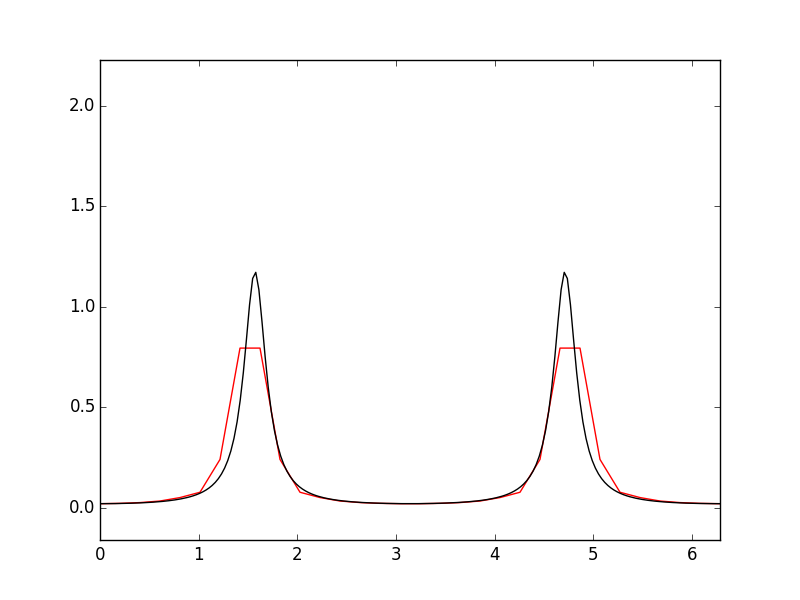
\includegraphics[width=0.43\textwidth]{./images/half_density_sqr_t1_00.png}
  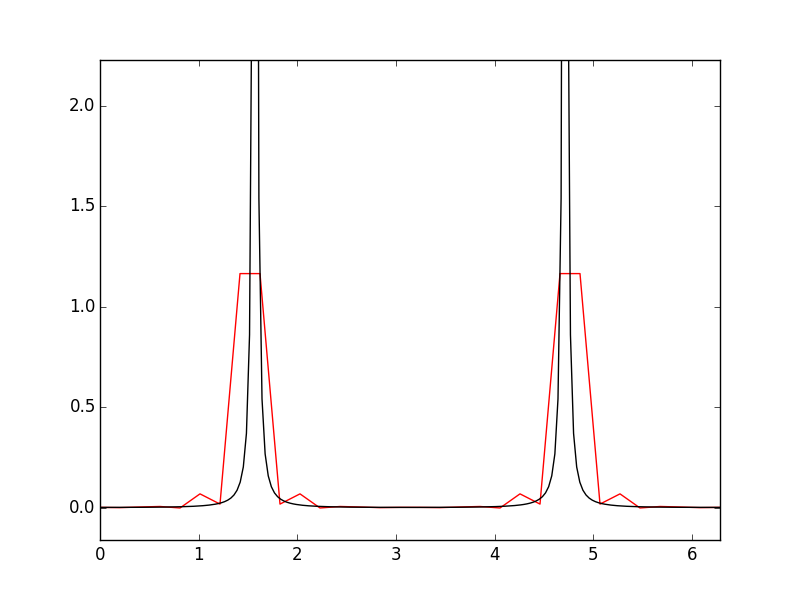
\includegraphics[width=0.43\textwidth]{./images/half_density_sqr_t2_00.png}
  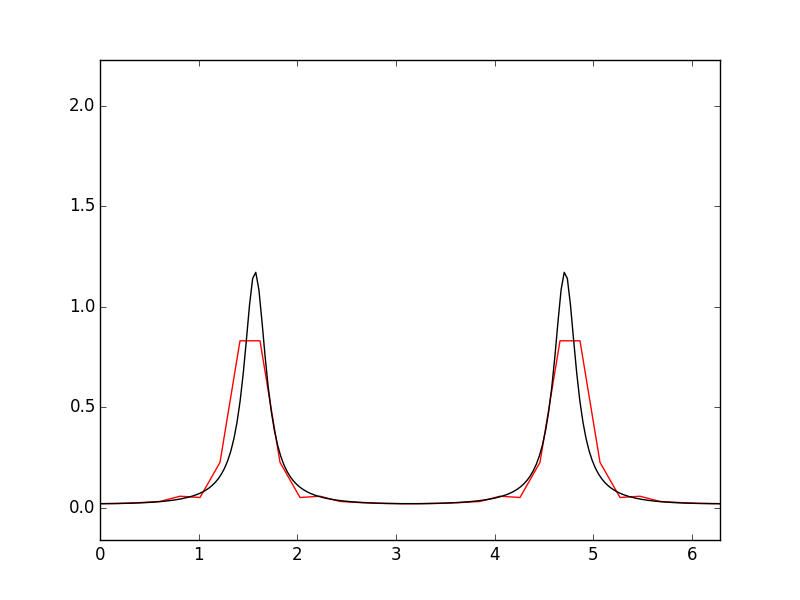
\includegraphics[width=0.43\textwidth]{./images/transfer_op_t1_00.png}
  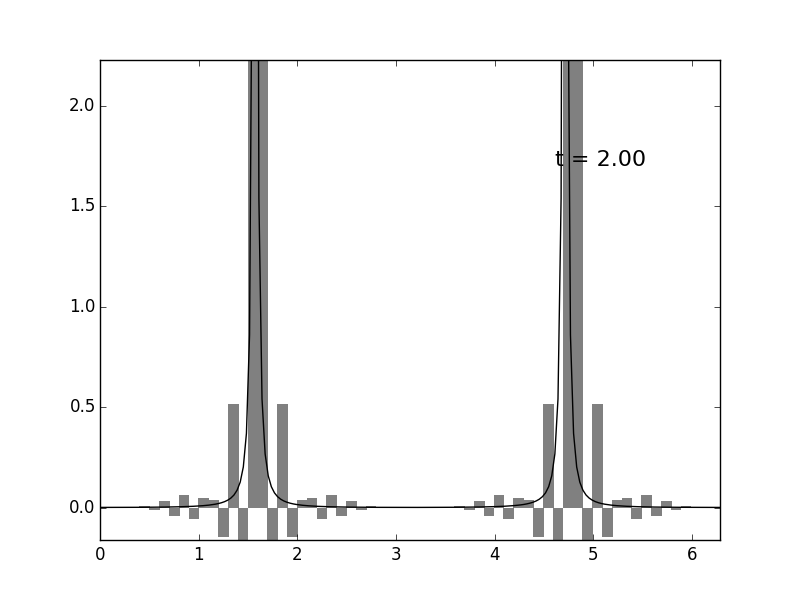
\includegraphics[width=0.43\textwidth]{./images/transfer_op_t2_00.png}
  \caption{Computed densities via our method and the transfer operator method with respect to the vector field $\dot{x} = \sin(2x)$ and with a uniform density at $t=0$.  The top two panels depict solutions computed with our scheme at time $t=1$ and $t=2$.   The bottom two panels depict the densities computed via transfer operator theory.  In each panel, the exact solution is plotted in black.}
  \label{fig:one_dim_system}
\end{figure}

\subsection{The Van der Pol oscillator}
Consider the system on $\R^2$ given by the ODE
\begin{align}
  \begin{split}
    \dot{x} &= y \\
    \dot{y} &= (1-x^2)y-x
   \end{split} \label{eq:vdp}
\end{align}
The vector-field is depicted in figure \ref{fig:vdp_quiver}.
\begin{figure}[p]
  \centering
  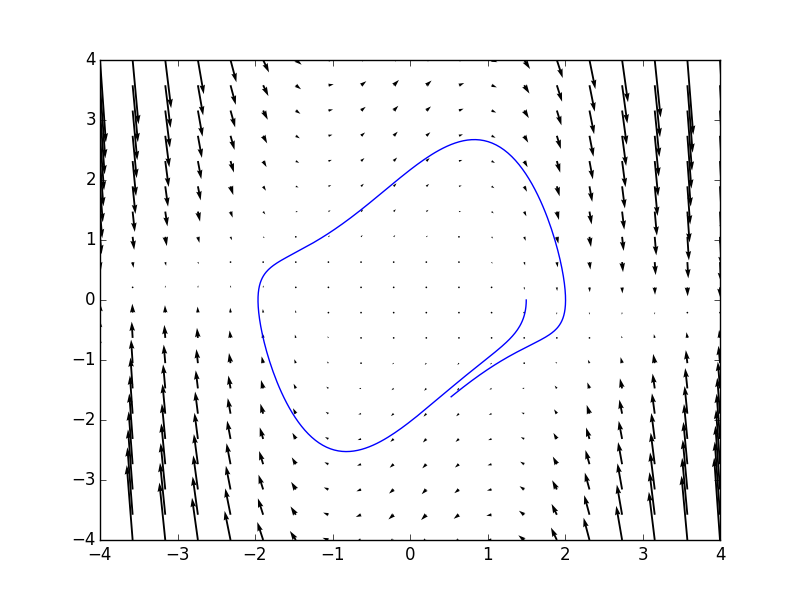
\includegraphics[width=0.5\textwidth]{./images/vdp_traj.png}
  \caption{A quiver plot of the vector-field given by \eqref{eq:vdp}.  The trajectory with initial condition (1.5,0) is shown in blue.}
  \label{fig:vdp_quiver}
\end{figure}

This vector field is particularly difficult for multiple reasons.
Firstly, the system is on a noncompact domain, so we are unable to
resolve the full domain using a finite set of basis functions.
Secondly, if we restrict ourselve to a compact subset, the boundary conditions are non-vanishing.  Even worse, they are a mixture of inflowing
and outflowing.
Finally, the system exibits a limit cycle.
As densities are attracted towards the limit cycle, they are 
exponentially flattened.  Eventually the density will flatten 
into a length scale below that which we've resolved.

Despite these problems on the boundaries, and with the resolution,
we are still able to construct a scheme which works on small times
in regions near the origin.
We consider a basis generated by Debauchies wavelets,
on the domain $[-8,8] \times [-8,8]$ with finest scale $2^{-3}$.
\todo[inline]{hoj:  You'll probably need to elaborate on this Ram.}
A typical advection is shown in 
figure \ref{fig:vdp_advection}.
One can see the density begin to hug the side of the limit cycle
at time $t=1$.


\begin{figure}[p]
  \centering
  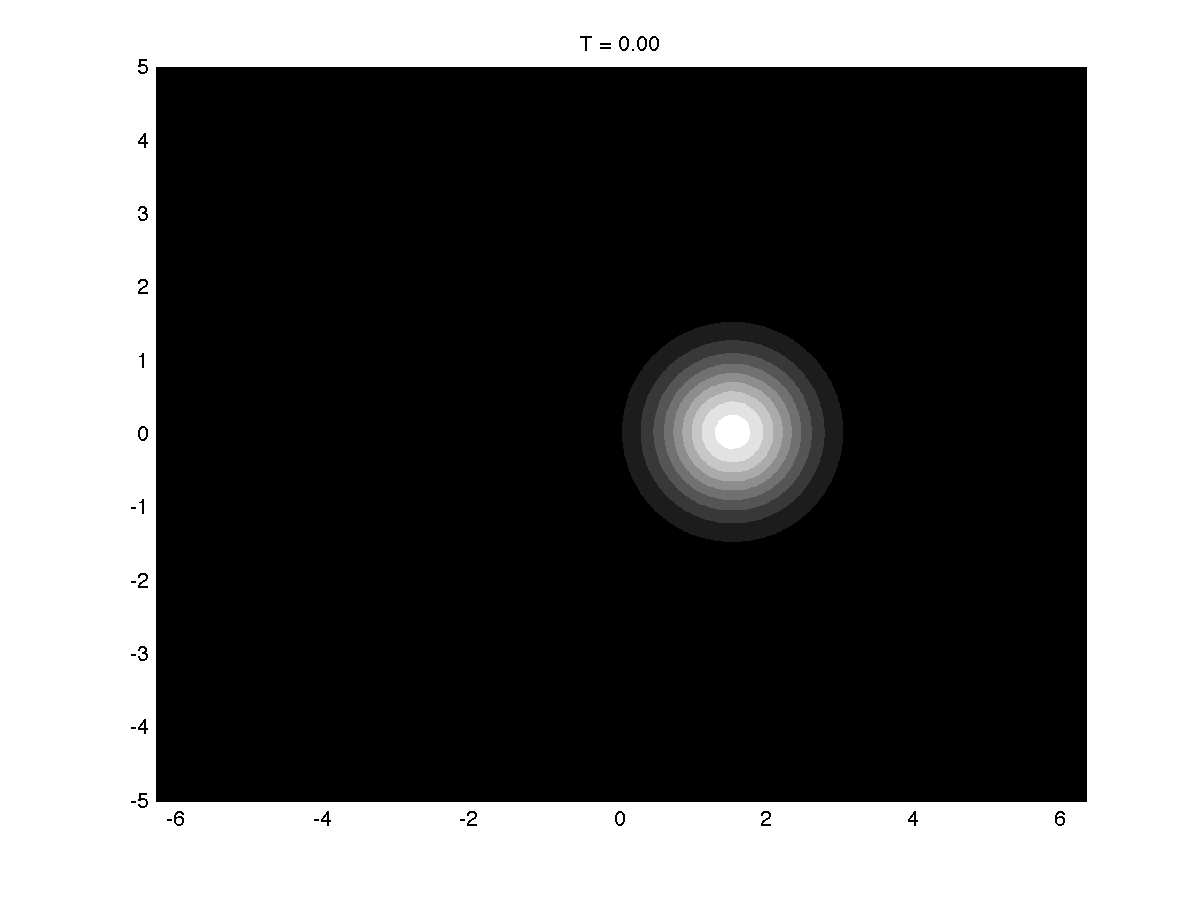
\includegraphics[width=0.43\textwidth]{./images/vdp_t0p0.png}
  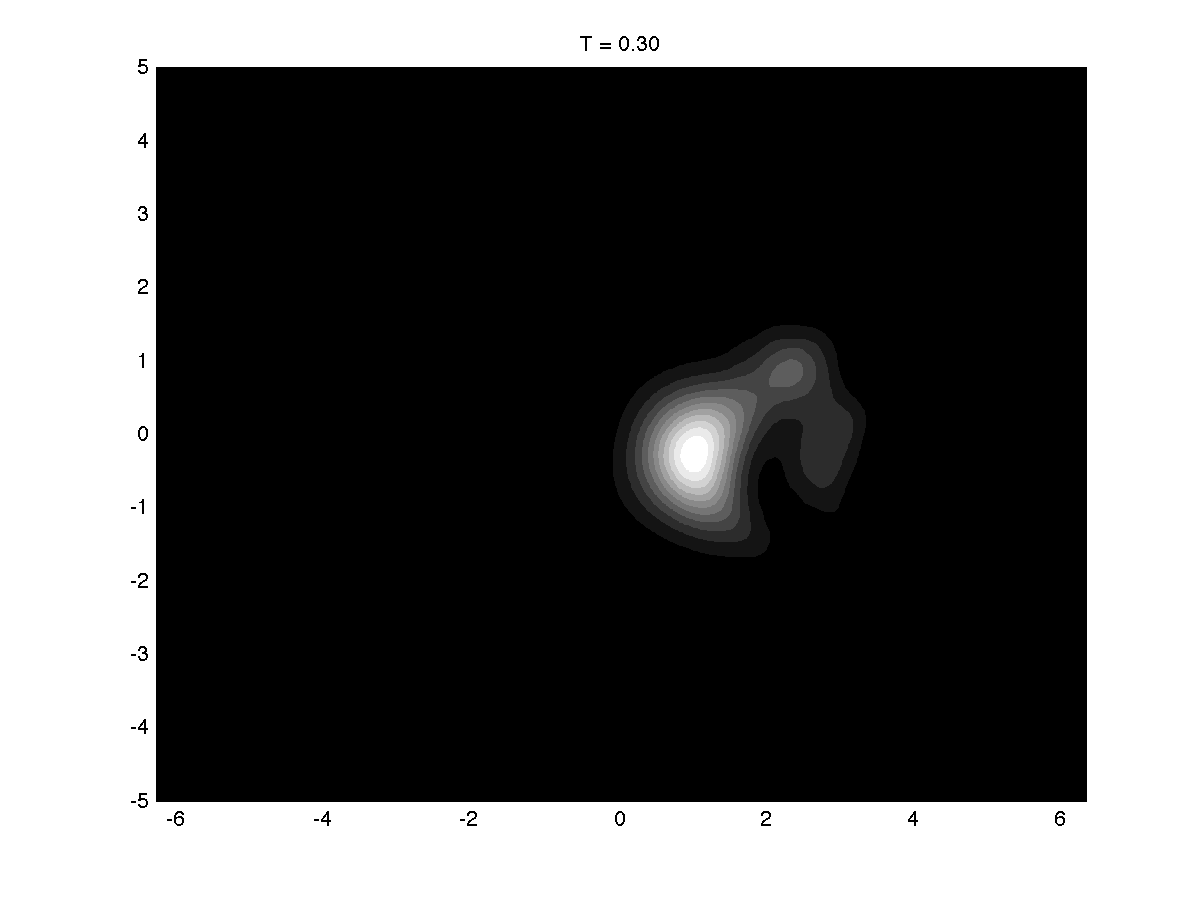
\includegraphics[width=0.43\textwidth]{./images/vdp_t0p30.png}
  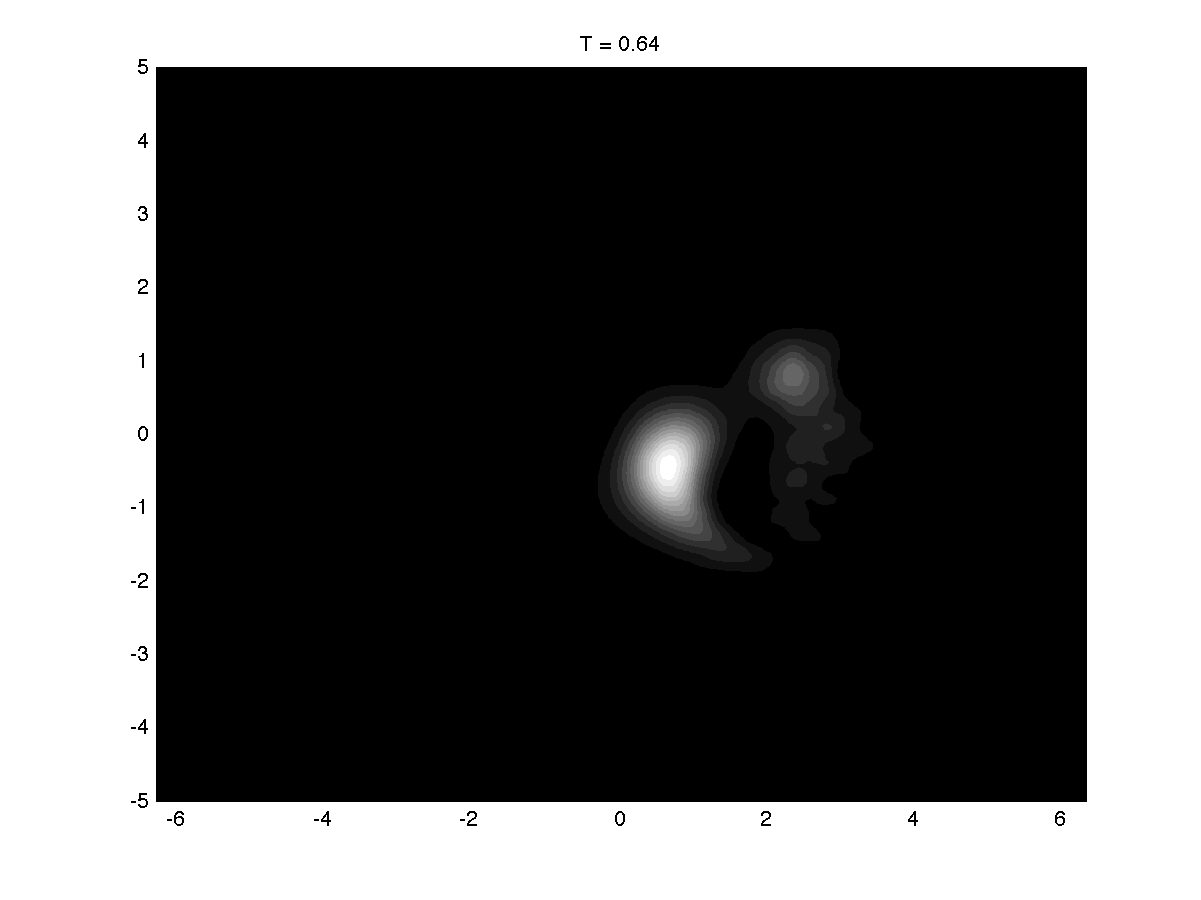
\includegraphics[width=0.43\textwidth]{./images/vdp_t0p64.png}
  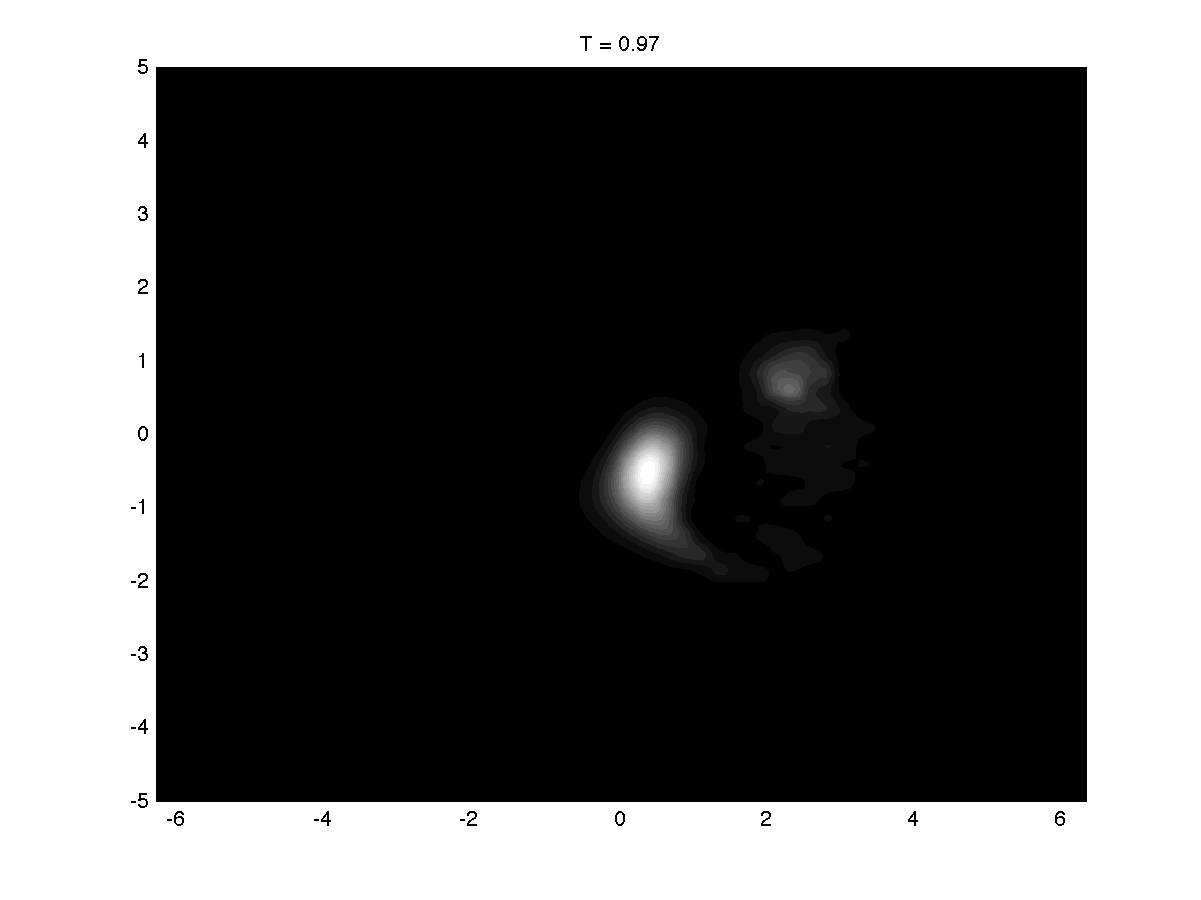
\includegraphics[width=0.43\textwidth]{./images/vdp_t0p97.png}
  \caption{Computed densities given a Gaussian initial condition
    and advected by \eqref{eq:vdp}.
    Snapshots are displayed at time $t=0.00,0.30,0.64,0.97$.
  }
  \label{fig:vdp_advection}
\end{figure}

\subsection{The rigid body equations}
In the absence of external forces
the equations of motion for the angular momentum, $\Pi \in \R^3$,
of a rigid body are
\begin{align}
  \dot{Pi} = \Pi \times ( \mathbb{I}^{-1}\cdot \Pi),  \label{eq:rigid_body}
\end{align}
where $\mathbb{I} = {\rm diag}(I_1,I_2,I_3)$,
and $I_1,I_2,I_3 > 0$ are rotational inertias along
the principal axes of rotation.
As $\dot{\Pi}$ is orthogonal to $\Pi$, we observe that
$\| \Pi \|$ is constant.  Thus the dynamics are constrained
to spheres.  Moreover, the dynamics on a sphere of radius $r>0$
are identical to the dynamics on a sphere of unit radius
upon rescaling time by $r^{-2}$.
Therefore we may (literally) restrict our analysis of this system
to an ode on the unit sphere $S^2 \subset \R^3$.
In spherical coordinates, the dynamics are given by
\begin{align*}
  \dot{\phi} &= -\sin^2(\phi) \cos(\theta) \frac{I_3-I_2}{I_3I_2}
  + \cos^2(\phi) \cos(\theta) \frac{I_1 - I_3}{I_1 I_3} \\
  \dot{\theta} &= - \sin(\theta) \sin(\phi) \cos(\phi) \frac{I_2 - I_1}{I_2I_1} \\
  \dot{r} &= 0
\end{align*}
A plot of various trajectories on $S^2$ is depicted in figure \ref{fig:rigid_body_traj}.

\begin{figure}[p]
  \centering
  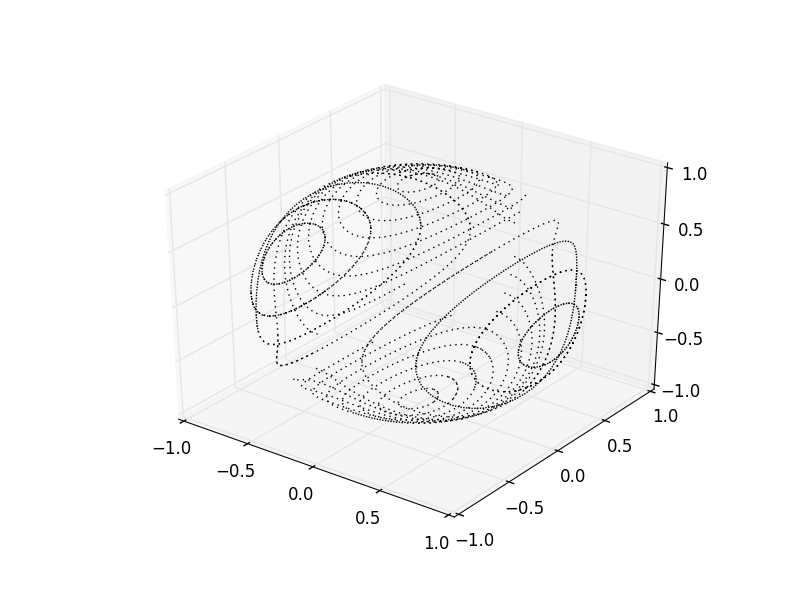
\includegraphics[width=0.8\textwidth]{./images/rigid_body_traj.png}
  \caption{trajectories of \eqref{eq:rigid_body} on the unit sphere.}
  \label{fig:rigid_body_traj}
\end{figure}

We can consider the global chart induced by spherical coordinates.
Specifically, this is the chart with
\begin{align*}
  U = S^2 \backslash (0,0,-1) \quad,\quad
  V = (0,\pi) \times (-\pi,\pi) \quad,\quad
  \varphi(\theta,\phi) = \begin{pmatrix}
    \cos(\phi) \sin(\theta) \\
    \sin(\phi) \sin(\theta) \\
    \cos(\theta)
    \end{pmatrix}.
\end{align*}
We may approximate $C^0(V)$ using the Haar wavelet,
and then push-forward these approximations
to obtain an advection scheme on $S^2$.


\section{Conclusion}

\hoj{Control systems.  Noise.  Manifolds with boundary.
  Adaptivity, and decreased regularity.}

\subsection{Acknowledgements}
Erica Kim (matlab + graphics help).
Richard Montgomery via Math Overflow (dense chart question).
Darryl Holm (applications to imaging)

\bibliographystyle{IEEEtran}
\bibliography{./hoj_2014}

\end{document}
